\documentclass[11pt,a4paper]{article}
\usepackage[top=3cm, bottom=2cm, left=3cm, right=2cm]{geometry}
\usepackage[utf8]{inputenc}
\usepackage{amsmath, amsfonts, amssymb}
\usepackage[brazil]{babel}
\usepackage[dvipsnames, svgnames]{xcolor}
\usepackage{tcolorbox}
\usepackage{tikz}
\usepackage{LobsterTwo}
\usepackage[T1]{fontenc}
\usepackage{fontspec}
\usepackage{txfonts}
\usepackage{titlesec}
\usepackage{varwidth}



\usepackage{lipsum}

\usetikzlibrary{patterns}
\tcbuselibrary{breakable}
\usetikzlibrary{shadings}

\tcbuselibrary{raster}
\tcbuselibrary{skins}
\tcbuselibrary{listings}
\tcbuselibrary{theorems}
\tcbuselibrary{hooks}
\tcbuselibrary{vignette}
\tcbsetforeverylayer{autoparskip}

\newsavebox\mysavebox

\tcbset{enhanced,colback=yellow!10,
colframe=DarkTurquoise!60!white,fonttitle=\LobsterTwo\Huge, coltitle=CarnationPink}

\titleformat{\tilte}{\LobsterTwo\LARGE\color{CarnationPink}}{\thetitle}{1em}{}
\titleformat{\section}{\LobsterTwo\LARGE\color{CarnationPink}}{\thesection}{1em}{}
\titleformat{\subsection}{\LobsterTwo\LARGE\color{CarnationPink}}{\thesubsection}{1em}{}

\title{\textcolor{CarnationPink}{\LobsterTwo\Huge{Mapa Mental}}}
\author{Dalila}
\date{}
\begin{document}
    \maketitle


    \begin{tcboxedraster}[raster columns=2, raster rows=4]
        {title=Boxed Raster}
        \begin{tcbitemize}[raster rows=4,raster height=7cm, raster every box/.style={colframe=red!50!black,colback=red!10!white}]
            \tcbitem[colframe=MediumOrchid!50!white,colback=MediumOrchid!10!white,raster multirow=4]
            multirow=4
            \tcbitem[raster multicolumn=1,raster multirow=4,blankest]
                \begin{tcbitemize}[raster rows=4,raster columns=1,raster height=\tcbtextheight]
                    \tcbitem[colframe=RubineRed!50!white,colback=RubineRed!10!white]
                    \tcbitem[colframe=RubineRed!50!white,colback=RubineRed!10!white]
                    \tcbitem[colframe=RubineRed!50!white,colback=RubineRed!10!white]
                    \tcbitem[colframe=RubineRed!50!white,colback=RubineRed!10!white]
                \end{tcbitemize}
        \end{tcbitemize}
    \end{tcboxedraster}

\newtcbox{\headline}[1][]{enhanced,center, ignore nobreak,fontupper=\LobsterTwo\Large,  colframe=DarkTurquoise!!white,colback=RubineRed!10!white, fuzzy shadow={0mm}{-1mm}{0mm}{0.1mm}%
{blue}, fuzzy shadow={1mm}{-1mm}{0mm}{0.1mm}{red}, tikznode upper,#1}



\begin{tcboxeditemize}[raster equal height=rows, raster columns=3, size=small, blankest]{title=Boxed Raster}
    \tcbitem \headline{Important\\Headline} 
    \tcbitem \headline{Important\\Headline} 
    \tcbitem \headline{Important\\Headline} 
\end{tcboxeditemize}

\newtcolorbox{shadowbox}[1]{fuzzy shadow={-1.5mm}{-1.5mm}{0mm}{0.1mm}%
{blue}, fuzzy shadow={1.5mm}{-1.5mm}{0mm}{0.1mm}%
{red}, title={#1}}

\begin{shadowbox}{Sera que foi?}
    Num a de ver que deu!!!
\end{shadowbox}


\newtcolorbox{degradebox}[1]{enhanced, frame style={left color=DarkTurquoise!75!white,
right color=MediumOrchid!75!white}, title={#1}}


\begin{degradebox}{Será que foi?}
    AAAAA
\tcblower
\end{degradebox}



\newtcolorbox{smallbox}[1]{enhanced, size=small, adjusted title=center,halign=center, underlay={\tcbvignette{size=4.5mm, outside node=frame,north style=CarnationPink,east style=DarkTurquoise,
south style=Melon,west style=MediumOrchid}}, title={#1}}


    \begin{tcbraster}[raster columns=2, raster equal skip=10mm, raster equal height, raster halign = center, raster valign = bottom, center title]
        \begin{smallbox}{Deus}
            Ola Meu Pai
        \end{smallbox}
        \begin{smallbox}{Deus}
            Ola Meu Pai
        \end{smallbox}
    \end{tcbraster}



\newenvironment{myitemize}{%

\begin{itemize}}{\end{itemize}}
\tcolorboxenvironment{myitemize}{blanker,
before skip=6pt,after skip=6pt,
borderline west={0.75mm}{0mm}{CarnationPink},
borderline west={0.75mm}{0.75mm}{DarkTurquoise},
borderline west={0.75mm}{1.5mm}{Melon},
borderline west={0.75mm}{2.25mm}{MediumOrchid}}

\begin{myitemize}
\item Alpha
\item Beta
\item Gamma
\end{myitemize}


\newtcolorbox{mybox}[2][]{enhanced, sidebyside, righthand width=5cm, skin=enhancedlast jigsaw,
    attach boxed title to top left={xshift=-4mm,yshift=-0.5mm},
    fonttitle=\LobsterTwo\Large,varwidth boxed title=2.0\linewidth,
    colbacktitle=DarkTurquoise!75!white,colframe=CarnationPink!75!white,
    interior style={top color=DarkTurquoise!10!white,bottom color=Melon!10!white},
    boxed title style={empty,arc=0pt,outer arc=0pt,boxrule=0pt},
    underlay boxed title={
        \fill[DarkTurquoise!45!white] (title.north west) -- (title.north east)
        -- +(\tcboxedtitleheight-1mm,-\tcboxedtitleheight+1mm)
        -- ([xshift=4mm,yshift=0.5mm]frame.north east) -- +(0mm,-1mm)
        -- (title.south west) -- cycle;
        \fill[MediumOrchid!90!white!] ([yshift=-0.5mm]frame.north west)
        -- +(-0.4,0) -- +(0,-0.3) -- cycle;
        \fill[Melon!90!white!] ([yshift=-0.5mm]frame.north east)
        -- +(0,-0.3) -- +(0.4,0) -- cycle; },
        title={#2},#1}

\begin{mybox}{Aalalalalsasjdte}
\lipsum[2]
\tcblower
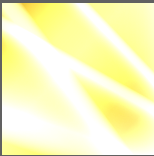
\includegraphics[width=\linewidth]{goldshade.PNG}
\end{mybox}




\end{document}